%%%%% for latexit

\documentclass[12pt]{article}
\usepackage{booktabs}
\usepackage[dvipsnames]{xcolor} %used for font color
\usepackage{amssymb} %maths
\usepackage{amsmath} %maths
\usepackage[utf8]{inputenc} %useful to type directly diacritic characters
\nopagecolor
\color{black!0.2}

\usepackage{tikz}
\usetikzlibrary{shapes,decorations,arrows,calc,arrows.meta,fit,positioning}
\tikzset{
    -Latex,auto,node distance =1 cm and 1 cm,semithick,
    state/.style ={ellipse, draw, minimum width = 0.7 cm},
    point/.style = {circle, draw, inner sep=0.04cm,fill,node contents={}},
    bidirected/.style={Latex-Latex,dashed},
    el/.style = {inner sep=2pt, align=left, sloped}
}


%%%%% distributions
\begin{tabular}{cccc}
    \toprule
    $H$ & $E$ & $C$ & $p(H,E,C)$\\
    \midrule
    0 & 0 & 0 & 0.47025 \\
    0 & 0 & 1 & 0.00495 \\
    0 & 1 & 0 & 0.004   \\
    0 & 1 & 1 & 0.4653  \\
    1 & 0 & 0 & 0.02475 \\
    1 & 0 & 1 & 0.00005 \\
    1 & 1 & 0 & 0.001   \\
    1 & 1 & 1 & 0.0297  \\
    \bottomrule
    \end{tabular}
    
    \begin{tabular}{c}
    \toprule
    $p(E=1)$\\
    \midrule
    $0.5$\\
    \bottomrule
    \end{tabular}
    
    \begin{tabular}{ccc}
    \toprule
    $E$ & $C$ & $p(H=1|E,C)$\\
    \midrule
    0 & 0 & 0.05       \\
    0 & 1 & 0.01       \\
    1 & 0 & 0.2        \\
    1 & 1 & 0.06       \\
    \bottomrule
    \end{tabular}
    
    \begin{tabular}{cc}
    \toprule
    $E$ & $p(C=1|E)$\\
    \midrule
    0 & 0.01     \\
    1 & 0.99    \\
    \bottomrule
    \end{tabular}



%%%%% bayesian network

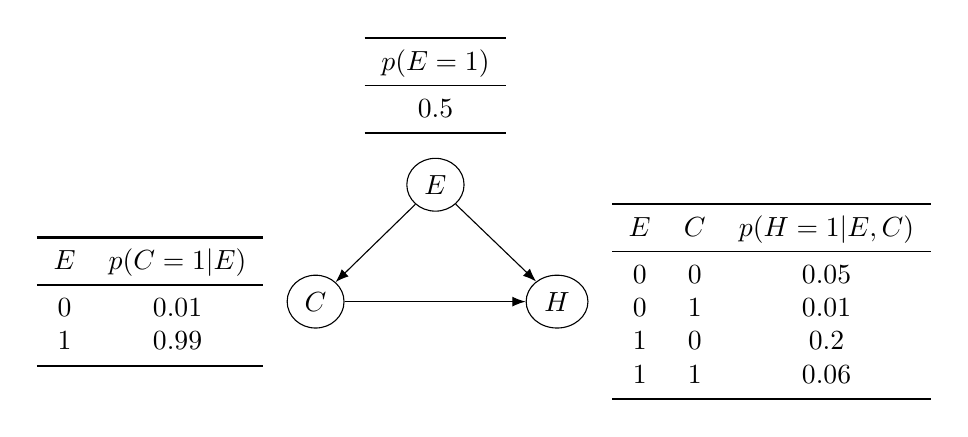
\begin{tikzpicture}
    % x node set with absolute coordinates
    \node[state] (E) at (0,0) {$E$};

    % y node set relative to x.
    % Locations can be:
    % right,left,above,below,
    % above left,below right, etc
    \node[state] (C) [below left =of E] {$C$};
    \node[state] (H) [below right =of E] {$H$};

    % Directed edge
    \path (E) edge (C);
    \path (E) edge (H);
    \path (C) edge (H);


\node [above=5pt of E]
{
\begin{tabular}{c}
\toprule
$p(E=1)$\\
\midrule
$0.5$\\
\bottomrule
\end{tabular}
};


\node [left=5pt of C]
{
\begin{tabular}{cc}
\toprule
$E$ & $p(C=1|E)$\\
\midrule
0 & 0.01     \\
1 & 0.99    \\
\bottomrule
\end{tabular}
};

\node [right=5pt of H]
{
\begin{tabular}{ccc}
\toprule
$E$ & $C$ & $p(H=1|E,C)$\\
\midrule
0 & 0 & 0.05       \\
0 & 1 & 0.01       \\
1 & 0 & 0.2        \\
1 & 1 & 0.06       \\
\bottomrule
\end{tabular}
};

\end{tikzpicture}